%\documentclass[letterpaper]{sig-alternate-10pt}
\documentclass[letterpaper]{sig-alternate-2013}
\usepackage{url,xspace,subfigure,multirow}
\usepackage{color,cite,graphicx}
\usepackage[font={small}]{caption}

%%% PG2013:: bunch of macros you can ignore them for now 
\def\full{0}        % set 1 for a full tech report version
                    % set 0 for submission version
\def\shownotes{1}   % set 1 for version with author notes
                    % set 0 for no notes
\def\anon{0}        % set 1 to anonymize
                    % set 0 for acks and author names

\def\showedits{1} %set for 1 to turn edits red, 0 for them to become black.

\newcommand{\namedref}[2]{#1~\ref{#2}}
\newcommand{\tableref}[1]{\namedref{Table}{#1}}
\newcommand{\sectionref}[1]{$\S$\ref{#1}}
\newcommand{\appendixref}[1]{\namedref{Appendix}{#1}}
\newcommand{\theoremref}[1]{\namedref{Theorem}{#1}}
\newcommand{\remarkref}[1]{\namedref{Remark}{#1}}
\newcommand{\definitionref}[1]{\namedref{Definition}{#1}}
\newcommand{\figureref}[1]{\namedref{Figure}{#1}}
\newcommand{\lemmaref}[1]{\namedref{Lemma}{#1}}
\newcommand{\claimref}[1]{\namedref{Claim}{#1}}
\newcommand{\propositionref}[1]{\namedref{Proposition}{#1}}
\newcommand{\constructionref}[1]{\namedref{Construction}{#1}}
\newcommand{\corollaryref}[1]{\namedref{Corollary}{#1}}
\newcommand{\equationref}[1]{\namedref{Equation}{#1}}
%
\newtheorem{theorem}{Theorem}[section]
\newtheorem{definition}[theorem]{Definition}
\newtheorem{lemma}[theorem]{Lemma}
\newtheorem{claim}[theorem]{Claim}
\newtheorem{proposition}[theorem]{Proposition}
\newtheorem{obs}[theorem]{Observation}
%

%%%%%%%  Author Notes %%%%%%%
%
\ifnum\shownotes=1
\newcommand{\authnote}[2]{{ $\ll$\textsf{\footnotesize #1 notes: #2}$\gg$}}
\else
\newcommand{\authnote}[2]{}
\fi
\newcommand{\Dnote}[1]{{\authnote{Dave}{#1}}}
\newcommand{\Anote}[1]{{\authnote{Abbas}{#1}}}
\newcommand{\Pnote}[1]{{\authnote{Phillipa}{#1}}}

%edits
\ifnum\showedits=1
\newcommand{\edit}[1]{\textcolor{red}{#1}}

\else
\newcommand{\edit}[1]{\textcolor{black}{#1}}
\fi

%%%%%%%%%%%%%%%%%%%%%%%%%%%%%%%%%

\providecommand{\vs}{vs. }
\providecommand{\ie}{\emph{i.e.,} }
\providecommand{\eg}{\emph{e.g.,} }
\providecommand{\cf}{\emph{cf.,} }
\providecommand{\resp}{\emph{resp.,} }
\providecommand{\etal}{\emph{et al. }}   %Removed trailing space here; usually want non-breaking space with following reference
\providecommand{\etc}{\emph{etc.}}      % No trailing space here either
\providecommand{\mypara}[1]{\smallskip\noindent\emph{#1} }
\providecommand{\myparab}[1]{\smallskip\noindent\textbf{#1} }
\providecommand{\myparasc}[1]{\smallskip\noindent\textsc{#1} }
\providecommand{\para}{\smallskip\noindent}


\title{Identifying Traffic Differentiation on Cellular Data Networks}
%\subtitle{subtitle (optional)}

\ifnum\anon=0

\author{
	\alignauthor Arash Molavi Kakhki$^\ddagger$, Abbas Razaghpanah$^\star$, Rajesh Golani$^\star$\\David Choffnes$^\ddagger$ , Phillipa Gill$^\star$, Alan Mislove$^\ddagger$ \\
	\affaddr{$\ddagger$Northeastern University, $\star$ Stony Brook University}
}


\else
\author{[Paper \#, X pages]}
\fi


\newfont{\mycrnotice}{ptmr8t at 7pt}
\newfont{\myconfname}{ptmri8t at 7pt}
\let\crnotice\mycrnotice%
\let\confname\myconfname%

\permission{Permission to make digital or hard copies of part or all of this work for personal or classroom use is granted without fee provided that copies are not made or distributed for profit or commercial advantage, and that copies bear this notice and the full citation on the first page. Copyrights for third-party components of this work must be honored. For all other uses, contact the owner/author(s). Copyright is held by the author/owner(s).}
\conferenceinfo{SIGCOMM'14,}{August 17--22, 2014, Chicago, IL, USA.} 
\copyrightetc{ACM \the\acmcopyr}
\crdata{978-1-4503-2836-4/14/08.\\
http://dx.doi.org/10.1145/2619239.2631445 }

\clubpenalty=10000 
\widowpenalty = 10000


\begin{document}
%% COPYRIGHT STUFF
%\iffalse
%\conferenceinfo{SIGCOMM'11,} {August 15-19, 2011, Toronto, Ontario, Canada.}
%\CopyrightYear{2011}
%\crdata{978-1-4503-0797-0/11/08}
%\fi

\clubpenalty=10000
\widowpenalty = 10000

\maketitle

%\section*{Abstract}
%{\it }

%% KEYWORDS. ACM classification system stuff. Feel free to ignore. 
\iffalse
\vspace{1mm}
\noindent
{\bf Categories and Subject Descriptors:} C.2.2
{[Computer-Comm\-uni\-cation Networks]}: {Network Measurement
}

\vspace{1mm}
\noindent
{\bf General Terms:}  Network Measurement, Mobile, Traffic Differentiation

%\vspace{1mm}
%\noindent
%{\bf Keywords:} Routing, BGP, Security
\fi

\section{Introduction}

%As wireless providers offer faster and more widely available cellular data to their customers, more mobile applications emerge that utilize this additional capacity to add more services to the mobile platform or improve on the quality of service for existing ones. However, it is often unclear how traffic from mobile services is treated while traversing boundaries of these networks. 

The goal of this research is to detect traffic differentiation in cellular data networks. We define service differentiation as any attempt to change the performance of network traffic traversing an ISP's boundaries. ISPs may implement differentiation policies for a number of reasons, including load balancing, bandwidth management, or business reasons. Specifically, we focus on detecting whether certain types of network traffic receive better (or worse) performance. As an example, a wireless provider might limit the performance of third-party VoIP or video calling services (or any other competing services) by introducing delays or reducing transfer rates to encourage users to use services provided by the wireless provider.

Previous work \cite{glasnost, zhang:netdiff, tariq:nano} explored this problem in limited environments. Glasnost focused on BitTorrent in the desktop/laptop environment, and lacked the ability to conduct controlled experiments to provide strong evidence of differentiation. NetDiff covered a wide range of passively gathered traffic from a large ISP but likewise did not support targeted, controlled experiments. We address these limitations with \textit{Mobile Replay}.

%Pevious efforts for detecting traffic differentiation include the Glasnost project, which focuses on identifying BitTorrent differentiation on broadband connections~\cite{glasnost}. However, Glasnost assumed a fairly stable underlying connection (broadband) and focused on a single application: BitTorrent, which required hand-tuning of the differentiation tests. In contrast, our approach aims to provide traffic differentiation testing regardless of the application being tested via a ``record-and-replay'' functionality. Further, our tool is designed with the high variability of mobile networks in mind when designing statistical measures to identify differentiation.

%Traffic differentiation is defined as tampering with the performance of the network done by the ISP in any shape or form. Service differentiation might be done for a variety of reasons. As an example, a wireless provider might limit the performance of third-party VoIP or video calling services (or any other competing services) by introducing delays or reducing transfer rates to encourage users to use services provided by the wireless provider. Also, a wireless provider might limit or disable traffic flow for file sharing applications, video streaming services, or other kinds of  "network-intensive" applications. These policies are often not disclosed to users or buried deep within fair usage policy sections of service contracts. For example, T-Mobile UK state in their data plan's fine print that VoIP is not allowed on their monthly cellular data plan.

%Service differentiation can be done based on host, port, and/or packet payload. As an example, an ISP could block all the connections that use port \texttt{4070} to block Spotify, reduce bandwidth for all traffic to and from \texttt{*.dropbox.com} for Dropbox, and block all the packets that appear to contain BitTorrent payloads (regardless of host/port). In this work, we use Meddle and develop an \emph{application agnostic} method for recording and replaying network traces to identify service differentiation in mobile networks\cite{meddle}.

%Previous efforts for detecting traffic differentiation include the Glasnost project, which focuses on identifying BitTorrent differentiation on broadband connections~\cite{glasnost}. However, Glasnost assumed a fairly stable underlying connection (broadband) and focused on a single application: BitTorrent, which required hand-tuning of the differentiation tests. In contrast, our approach aims to provide traffic differentiation testing regardless of the application being tested via a ``record-and-replay'' functionality. Further, our tool is designed with the high variability of mobile networks in mind when designing statistical measures to identify differentiation.

%Previous work on detecting service differentiation worked on home ISPs and not mobile networks, this is covered in Section~\ref{sec:prevwork}. The Glasnost project worked on detecting differentiation of BitTorrent traffic in home ISPs using a browser applet. Our approach will test cellular networks for differentiation on a set of suspected services using Meddle VPN. Our methodology is explained in section~\ref{sec:method}.
%
%\section{Previous Work}
%\label{sec:prevwork}

%Glasnost and Meddle.
%In a previous effort to detect service differentiation, the Glasnost project made a web-based tool that users could use to see if their ISPs differentiates their traffic. Glasnost detects service differentiation for BitTorrent and does so by comparing metrics for a "reference" flow and "BitTorrent" flow over BitTorrent ports.

%Glasnost makes a connection to a measurement server's BitTorrent port and sends BitTorrent traffic, then it sends the same amount of data to the same server, only this time the data does not look like BitTorrent data. This process is repeated many times both on on BitTorrent ports and on other ports. Then the metrics calculated are compared to see if BitTorrent flow is being treated differently. This way, Glasnost can identify differentiation based on port and/or content.

%\begin{figure}[ht]
%\centering
%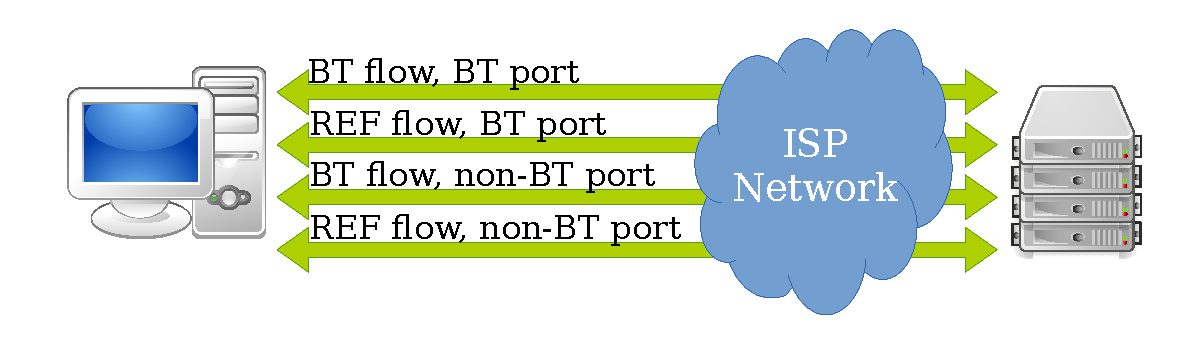
\includegraphics[width=3.3in]{figures/glasnost}
%\caption{Schematic view of how glasnost works.}
%\label{fig:glasnost}
%\end{figure}

%This measurement can be performed by logging into Glasnost test page and loading the Java\texttrademark applet. This design will not allow mobile devices to run the test as mobile devices can not run Java applets in their web browsers. Additionally, Glasnost is designed only to detect BitTorrent traffic differentiation.

\section{Mobile replay}
\label{sec:method}

%\subsection{Assumptions} 
We assume that ISPs will differentiate traffic based on hostname, IP addresses, ports, total number of connections, payload signatures, total bandwidth and time of day. Our system currently can detect all of these forms of differentiation with the exception of server-based differentiation.

\subsection{Overview} Mobile Replay identifies service differentiation using two key components. First, it tests for differentiation by replaying real network traces generated from user interactions with apps. Meddle \cite{meddle} facilitates capturing this information, and we develop new strategies for replaying arbitrary app traces. Second, Mobile Replay exploits the Meddle VPN to conduct controlled experiments. By alternately replaying traffic over tunneled and untunneled connections multiple times in rapid succession, we control for factors that ISPs may use to differentiate traffic.

A key challenge is how to capture and replay the salient features of application traffic such that it will be subject to differentiation from middleboxes. To this end, we design a system that captures traffic generated by users' devices (via Meddle) and replays those flows from a replay server. Another challenge is how to establish ground truth as to whether the ISP is differentiating service for replay traffic. To address this, we exploit the VPN connection that Meddle provides as follows. When the VPN is enabled, the ISP cannot inspect flow contents and thus cannot differentiate based on the above factors except total bandwidth and time of day. We then compare this performance to the case when we send traffic untunneled. Using multiple successive trials of tunneled and untunneled replay experiments, we can determine the noise inherent in performance metrics in each type of experiment (tunneled vs not tunneled), then identify cases where there are statistically significant differences between them -- indicating differentiation.

\begin{figure}[t]
\centering
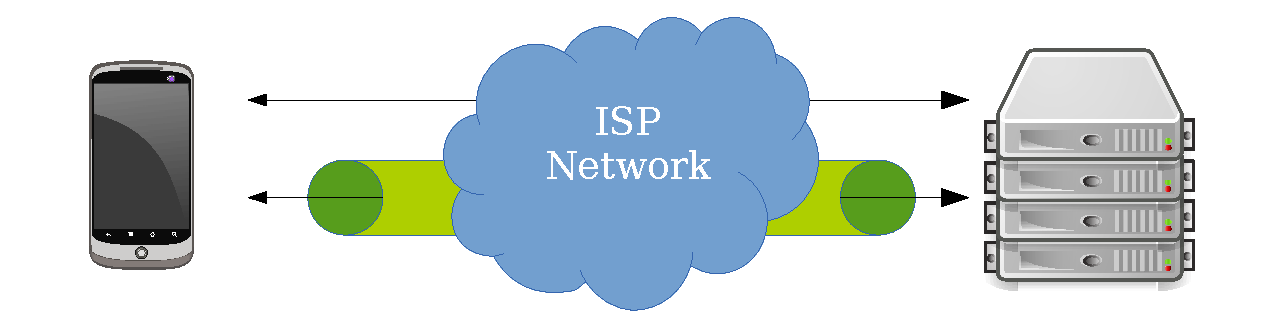
\includegraphics[width=3.5in]{figures/meddle}
\vspace{-0.5cm}
\caption{Schematic view of how our project works. Traffic is sent unencrypted and through the Meddle VPN tunnel between the mobile client and a control server.}
\label{fig:meddle}
\end{figure}

\subsection{Replay and methodology}
We support both UDP and TCP flows in our replay system, which consists of a client app running on the mobile device and a replay server written in Python in a event-driven fashion using Gevent \cite{gevent}, which performs efficiently with many concurrent clients. The server also performs UDP hole punching to support clients behind a NAT. The client and server coordinate to replay the original flows to reproduces packet timings, sequence of bytes, ports and client IPs. Since our replay is limited to using our own replay servers, we cannot detect differentiation based on arbitrary server IPs (a topic of ongoing work). \edit{Note, however, that if our replay servers are co-located with servers contacted in our traces, we do not suffer from this limitation. For example, if we use EC2 servers and the tested app streams video from a server in the same data center (and/or same block of IP addresses), we may be able to trigger the same differentiation in our replays.}

We detect differentiation according to the following metrics. First, we compute checksums to verify that the bytes sent/received at each endpoint during the replay are exactly the same as the original trace. If not, we flag a case of content manipulation/blocking. Second, we compute summary statistics on throughput, loss, and RTT. Unlike manipulation/blocking, there are confounding factors other than differentiation that may causes changes in these statistics between the record and replay.
To address this issue, we run multiple replay trials (10 total\edit{, though we are investigating dynamically adjusting the number of trials in response to observed noise}), alternating between using a VPN connection ($R_T$) and an untunneled one ($R_U$). By computing statistics over multiple trials of one category ($R_T$ or $R_U$) we can quantify natural variations in performance that are not a result of differentiation. Having computed the variance over $R_T$ and $R_U$, we can compare the summary statistics (mean/median) of $R_T$ and $R_U$ and use the variance in each category to determine if the differences are statistically significant.
Note that ISPs may apply differentiation to all VPN traffic, e.g., by throttling. To detect this, we group all $R_T$ samples and compare them to all $R_U$ samples across all applications and use the analysis described above.

\begin{figure}[t]
	\centering
%	\vspace{-0.25in}
	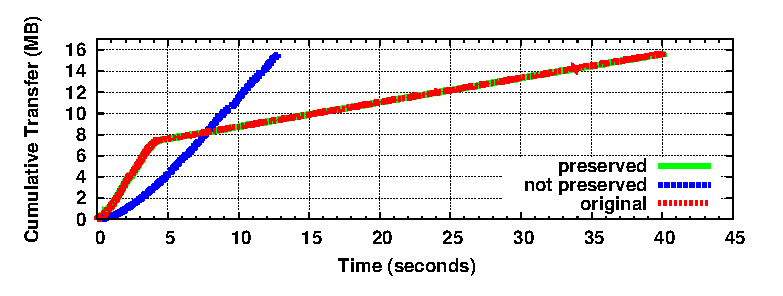
\includegraphics[width=3.25in]{figures/double.eps}
	\caption{Cumulative byte-transfer plot of YouTube trace replays with inter-packet timing preserved vs. not preserved. The x-axis is time and y-axis is the total number of bytes transferred to that point. Observe that the original packet trace looks identical to the replay when timing is preserved. }
	\label{fig:double}
%	\vspace{-1em}
\end{figure}


\subsection{Feasibility}
We now demonstrate that our replay module performs as expected and can detect differentiation.
% Figure \ref{fig:nfx_double} uses a sequence-number diagram to compare the behavior of original traces to those generated by our replay system, in an environment where we know differentiation is not happening.

By preserving packet ordering and timing, our system produces very similar results to the original traffic. Figure \ref{fig:double} shows a YouTube trace replayed in both conditions side-by-side. Of course, a variety of factors can differ between record and replay, including network conditions and access technology. In particular, apps may change their behavior in response to network technology and available bandwidth. In such cases, we must ensure that we replay traffic that was originally captured over similar network conditions. In our experiments, YouTube was the only app that exhibited such behavior.

We next tested whether we can detect differentiation in a controlled environment. We ran a full replay test with YouTube in a test environment where we \edit{inject a simple form of} differentiation by adding a 3\% packet loss and 10ms of delay. Figure \ref{fig:diff} shows CDFs of throughput during the replays, with and without differentiation. \edit{The effect of differentiation on the distribution is clear}, indicating that our system and metrics allow us to distinguish between differentiation and noise. Last, we tested our approach using several application traces on Verizon in Boston. Figure \ref{fig:nodiff} shows our replay results for two of those services, and we are able to confirm that there is no differentiation.

%A few qualities had to be verified about reference service trace: the reference WiFi network on which the packets were recorded should be well provisioned itself (i.e. no service differentiation mechanism should be in place), so the traces were recorded on campus WiFi network. Additionally, tested applications shouldn't behave differently on WiFi compared to when they are on cellular network. This was confirmed for all tested applications by recording traces once on a WiFi network and an HSDPA+ network with roughly the same bandwidth.

%\begin{figure}[t]
%	\centering
%	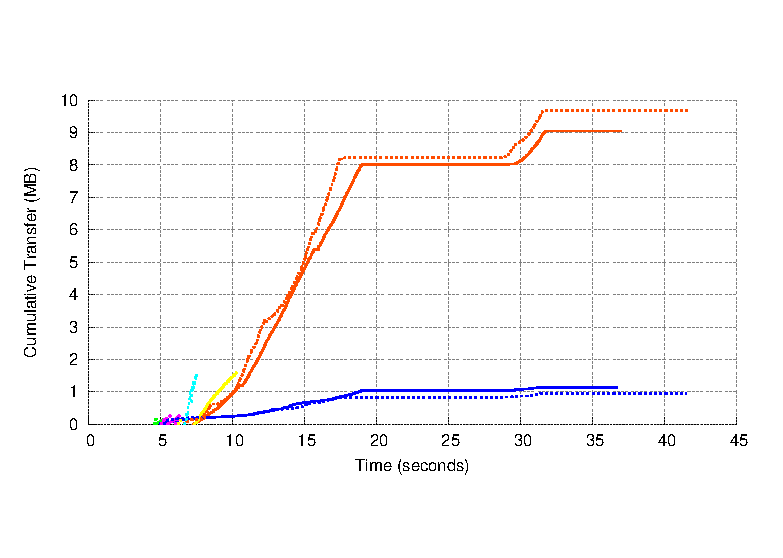
\includegraphics[height=1.3in]{figures/netflix_seqnum_wifi_vs_cell}
%	\caption{Plot of record (solid) and and replay (dashed) from Netflix activity. The x-axis is time and y-axis is the total number of bytes transferred to that point.}
%	\label{fig:nfx_double}
%\end{figure}


\begin{figure}[t!]
	\centering
	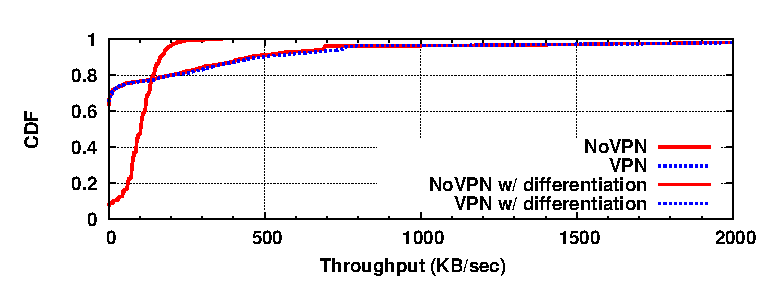
\includegraphics[width=3.25in]{figures/diff_no_diff.eps}
	\caption{CDF of throughput over time, with and without extra delay and packet loss induced at the server. 
	Our approach allows us to detect differences in throughput sample distributions when differentiation is applied. }
	\label{fig:diff}
%	\vspace{-1em}
\end{figure}

%\begin{figure}[t!]
%	\centering
%	\includegraphics[width=\linewidth]{figures/others2.png}
%	\caption{CDF of throughput over time left: Netflix, right: Pandora}
%	\label{fig:nodiff}
%%	\vspace{-1em}
%\end{figure}

\begin{figure}[h]
\centering
\vspace{0.2in}
\subfigure[ ]{\epsfig{figure=figures/nfx.eps,width=1.55in}\label{fig:a}}
\subfigure[ ]{\epsfig{figure=figures/spotify.eps,width=1.55in}\label{fig:b}}
\caption{CDF of throughput over time for Verizon (left: Netflix, right: Spotify). \edit{Our tests show 
that Verizon does not differentiate traffic for these apps.} }
\label{fig:nodiff}
\end{figure}


%Because the reference packet traces were recorded on a WiFi network with significantly higher bandwidth, this would have no effect on the outcome of the tests because this wouldn't affect the differentiation.

%\begin{figure}[ht]
%\centering
%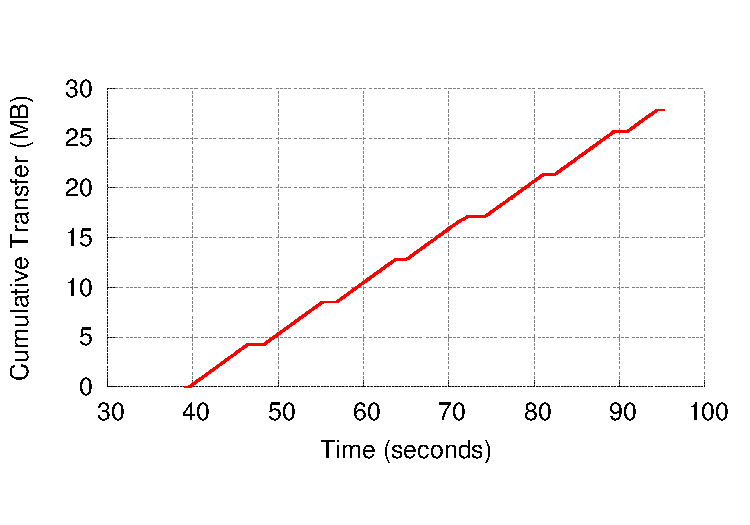
\includegraphics[width=3.3in]{figures/db_big_u}
%\caption{Sequence number plot for a connection made during a Dropbox upload session on WiFi showing application-level flow control.}
%\label{fig:dbu}
%\end{figure}


%\begin{figure}[t!]
%	\centering
%	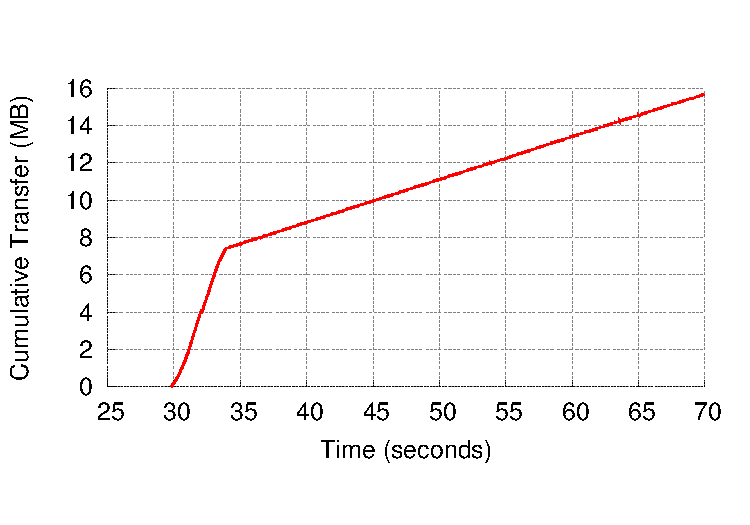
\includegraphics[width=0.45\textwidth]{figures/ytd}
%	\vspace{-0.8cm}
%	\caption{Sequence number plot for a connection made during a YouTube video session on WiFi showing application-level flow control.}
%	\label{fig:youtube}
%\end{figure}

%\subsection{Noise Packets}

%A smartphone that is connected to the Internet will always send and receive packets due to the services and applications that are running in the background (e.g. mail clients, update agents) so it was decided not to eliminate those packets because they were a natural part of what happens during a session.

%Although for the plots, the connections shown are the ones with the largest amount of transferred bytes. If the connection's total bytes transferred during a session multiplied by a threshold is larger than or equal to the connection with largest number of bytes transferred in that session, it will be in the plot. Figure~\ref{fig:tors} demonstrates this method.

%\begin{figure}[ht]
%\centering
%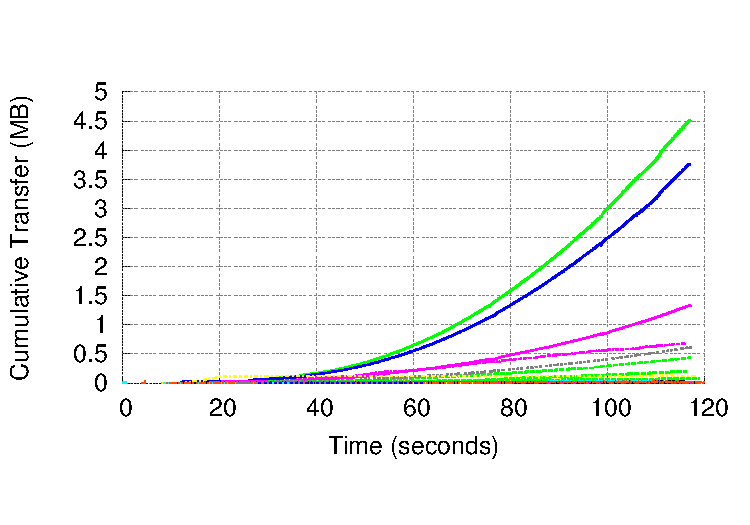
\includegraphics[width=3.3in]{figures/tor_nothr}
%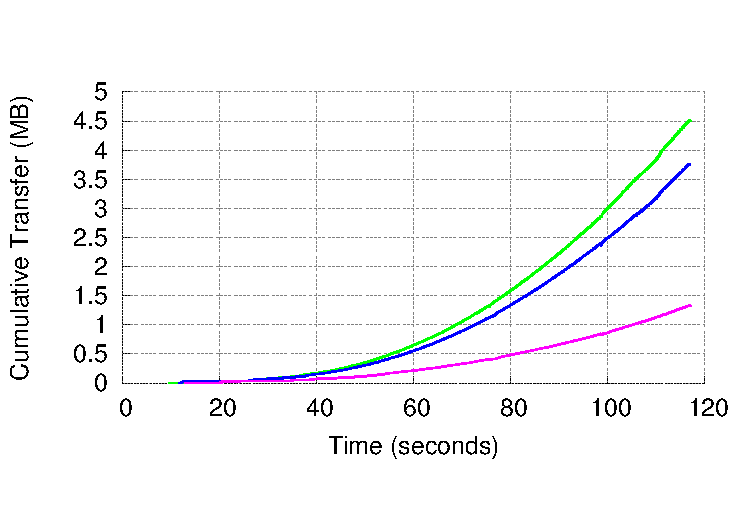
\includegraphics[width=3.3in]{figures/tor_thr}
%\caption{Sequence number plot for connections made during a BitTorrent session on WiFi. Top: without a cut-off threshold, Bottom: With a cut-off threshold of 4}
%\label{fig:tors}
%\end{figure}

%\noindent\textbf{Metrics.}
%Metrics calculated include, round-trip times (RTT), throughput, and loss rate. These metrics are calculated for both replays over both channels (encrypted (VPN) and unencrypted (no VPN)) and compared.% to detect differences.
%
%In cases that there are statistically significant differences between the metrics for a service, a differentiation mechanism is suspected to exist. This can be further investigated by other methods.

%\begin{figure}[ht]
%\centering
%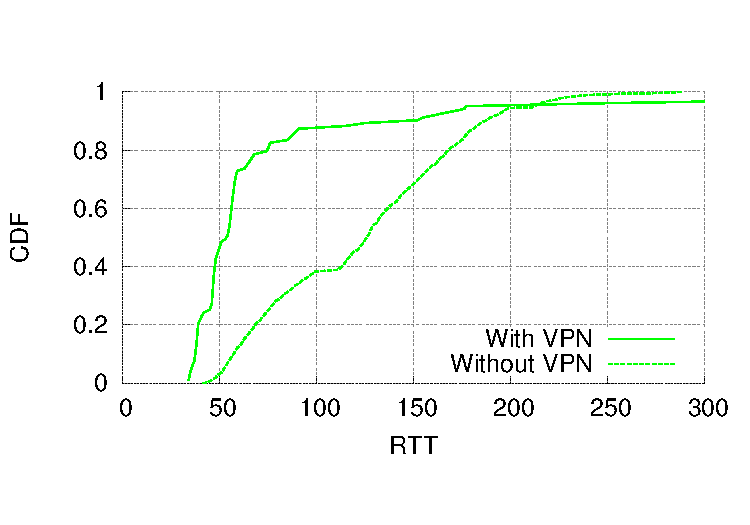
\includegraphics[width=3.3in]{figures/att_dbu_cdfrttp}
%\caption{CDF for RTT samples of YouTube upload sessions on AT\&T network show higher RTTs when not encrypted.}
%\label{fig:att_dbu}
%\end{figure}

%Note that some difference in throughput between encrypted and unencrypted replays is expected (and observed) because at the same bandwidth, a VPN connection will add overhead to the packets. But since this should decrease performance of the encrypted channel, it means that our differentiation detection will behave in a conservative manner.

%%PG: we fixed this ...
%Another reason for this maybe the processing carried out by the replay scripts to verify packets using hash functions.

%\begin{figure}[ht]
%\centering
%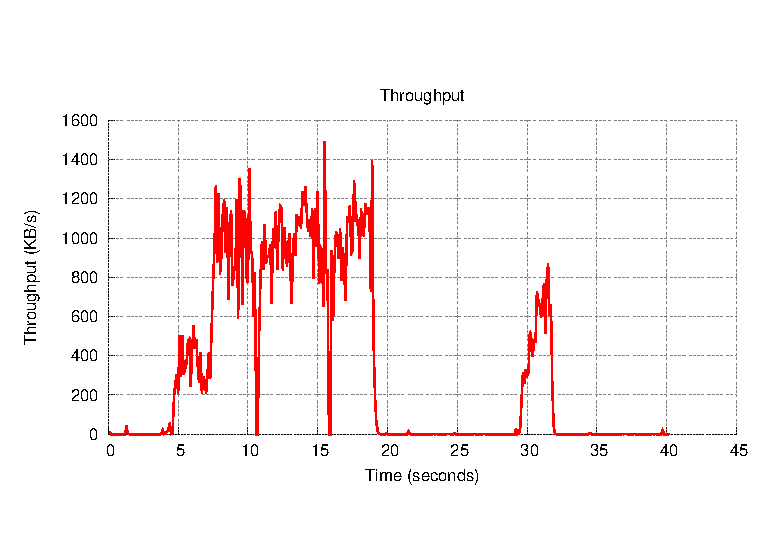
\includegraphics[width=3.3in]{figures/xp}
%\caption{Throughput calculated over 0.1 second intervals for a Spotify session on AT\&T. Throughput for the VPN connection is generally lower than that of the unencrypted connection.}
%\label{fig:xputs}
%\end{figure}

%\section{Preliminary Results}
%To evaluate our record and replay mechanism, tests were performed on a number of well-known wireless providers in North America. Figure~\ref{fig:res_bar} shows average throughput (with error bars indicating the standard deviation) from tests performed on Verizon's network. Based on these results, we cannot conclude that differentiation takes place in Verizon's network. We made similar observations in other networks measured in our preliminary study. Figure~\ref{fig:res_bar} also serves to highlight the challenge that network variability poses when detecting traffic differentiation in mobile networks. 

% These initial results do serve to highlight the challenges faced wh
%These results show that in fact there isn't a differentiation mechanism in their network for any of the tested services. Loss rates for all of the tests were within error margins.
% and results indicated that differentiation mechanisms are not in fact present in those networks.
%Also, as mentioned before, significantly different metrics in a network, while rising suspicion about its treatment of a certain type of traffic, will be inconclusive until complemented by further testing.


%\begin{table}
%\centering
%\begin{small}
%\setlength{\tabcolsep}{.01em}
%\begin{tabular}{|c|c|c|c|c|}
%\hline
%\multirow{2}{*}{\bf App}&\multicolumn{2}{c|}{\bf Throughput (KB/s)}& \multicolumn{2}{c|}{\bf Loss (\%)} \tabularnewline
%\cline{2-5}
%                             &{\bf No VPN} &{\bf VPN}&{\bf No VPN}&{\bf VPN}   \tabularnewline
%                             &{\bf (avg, stdev)} &{\bf (avg, stdev)}&{\bf (avg, stdev)}&{\bf (avg, stdev)}   \tabularnewline
%\hline
%
%YT(DL)&(103.74, 31.16)&(99.85, 35)&(0.81, 0.06)&(0.86, 0.13) \tabularnewline
%\hline
%YT(UL)&(114.52, 6.05)&(117.37, 8.78)&(0.03, 0.01)&(0.05, 0.01) \tabularnewline
%\hline
%DB(DL) &(155.09, 32.42)&(148.1, 44.95)&(0.79, 0.31)&(0.88, 0.38) \tabularnewline
%\hline
%DB(UL)&(115.07, 7.31)&(120.25, 5.85)&(0.07, 0.02)&(0.09, 0.01) \tabularnewline
%\hline
%SPTFY&(123.91, 40.19)&(127.16, 45.96)&(0.83, 0.08)&(0.73, 0.07) \tabularnewline
%%\hline
%%PNDR&(126.01, 36)&(122.81, 28.42)&(1.08, 0.09)&(1.13, 0.10) \tabularnewline
%\hline
%NFLX&(122.81, 28.42)&(132.26, 33.55)&(0.97, 0.03)&(0.99, 0.15) \tabularnewline
%\hline
%\end{tabular}
%\end{small}
%\caption{ \textbf{Average and standard deviation for 4  apps } \emph{(YT: YouTube, DB: Dropbox, SPTFY: Spotify, NFLX: Netflix; UL=Upload, DL=Download) on 
%Verizon. The differences in performance are within the noise, indicating no service differentiation. }}
%\label{tab:svcdiff}
%\end{table}

%\begin{figure}[t]
%\centering
%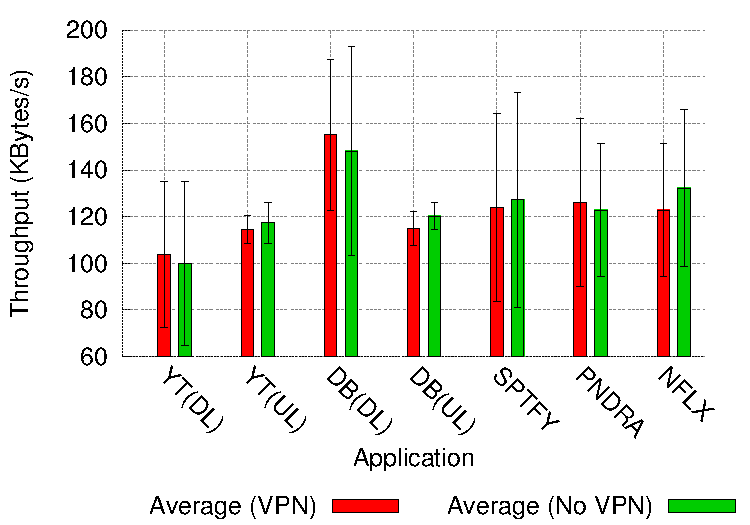
\includegraphics[width=0.45\textwidth]{figures/results}
%\caption{YT: YouTube, DB: Dropbox, SPTFY: Spotify, PNDRA: Pandora, NFLX: Netflix; UL=Upload, DL=Download) on Verizon. The differences in performance are within the noise, indicating no service differentiation.}
%\label{fig:res_bar}
%\end{figure}


\section{Future Work}

To address the limitation that we cannot detect differentiation based on server ports, our future work includes leveraging source-spoofing such that the source IP in the server's packets are the same as in the original traces. Additionally, because the VPN itself may be subject to differentiation (or blocked), we are investigating using multiple differentiation detection approaches, including randomizing packet payloads and ports in the replay.
%
%Currently, the testing and measurement is done on a laptop tethered to a phone by a researcher. 
\edit{We are also developing an app that allows average users to create and conduct tests from an mobile provider worldwide. We plan to use results from these tests to produce a Web site informing consumers of ISP policies.}
%%, as well as giving data to detect differentiation on newer ones.
%Additionally, our platform will reveal possible differentiation variations on the same network in different regions.

%% sample bib file with references.

\begin{small}
	\bibliographystyle{abbrv}
	\bibliography{oni}
\end{small}


\end{document}
